% add. options: [seceqn,secthm,crcready]
\documentclass[sw]{iosart2x}
%\usepackage[T1]{fontenc}
\usepackage{todonotes}
\usepackage{cleveref}
\usepackage{csquotes}
\usepackage{aurl}
\usepackage{booktabs}
\usepackage{tabulary}
%\usepackage{dcolumn}
%\usepackage{placeins} %provides \FloatBarrier

\newcommand{\aw}{AnthroWorks3D}
\newcommand{\anno}[1]{\href{https://annosaxfdm.de/ontology/#1}{\texttt{#1}}}
\newcommand{\gfo}[1]{\href{https://www.onto-med.de/ontologies/gfo/#1}{\texttt{#1}}}
\newcommand{\fma}[1]{\href{http://purl.org/sig/ont/fma/fma#1}{\texttt{#1}}}
\daurl{anno}{https://annosaxfdm.de/ontology/}
\daurl{gfo}{https://www.onto-med.de/ontologies/gfo\#}
\daurl{fma}{http://purl.org/sig/ont/fma/fma}
\daurl{ta2}{https://ta2viewer.openanatomy.org/?id=}

\pubyear{2023}
\volume{0}
\firstpage{1}
\lastpage{1}

\begin{document}

\begin{frontmatter}

%\pretitle{}
\title{The ANthropological Notation Ontology (ANNO): A core ontology for annotating human bones and deriving phenotypes}
\runtitle{Anthropological Notation Ontology}
%\subtitle{}

% For one author:
%\author{\inits{N.}\fnms{Name1} \snm{Surname1}\ead[label=e1]{first@somewhere.com}}
%\address{Department first, \orgname{University or Company name},
%Abbreviate US states, \cny{Country}\printead[presep={\\}]{e1}}
% Höffner, Heuschkel, Schmiedel, Penne, Fritzsch, Ludwig, Mohaupt, Labudde, Uciteli
% TODO: overleaf
% Two or more authors:
\begin{aug}
\author[B,C]{\inits{M.}\fnms{Marie} \snm{Heuschkel}\ead[label=e2]{marie.heuschkel@hs-mittweida.de}}
\author[A,C]{\inits{K.}\fnms{Konrad} \snm{Höffner}\ead[label=e1]{konrad.hoeffner@uni-leipzig.de}%
\thanks{Corresponding author. \printead{e1}.}
}
\author[B]{\inits{F.}\fnms{Fabian} \snm{Schmiedel}\ead[label=e3]{fabian.schmiedel@hs-mittweida.de}}
\author[B]{\inits{D.}\fnms{Dirk} \snm{Labudde}\ead[label=e10]{dirk.labudde@hs-mittweida.de }}
\author[A]{\inits{A.}\fnms{Alexandr} \snm{Uciteli}\ead[label=e11]{alexander.uciteli@imise.uni-leipzig.de}}
\address[A]{Institute for Medical Informatics, Statistics and Epidemiology (IMISE), \orgname{Leipzig University},
Saxony, \cny{Germany}\printead[presep={\\}]{e1,e11}}
\address[B]{\orgname{Hochschule Mittweida},
Saxony, \cny{Germany}\printead[presep={\\}]{e2,e3,e10}}
\address[C]{equal contribution}
\end{aug}

%\begin{review}{editor}
%\reviewer{\fnms{First} \snm{Editor}\address{\orgname{University or Company name}, \cny{Country}}}
%\reviewer{\fnms{Second} \snm{Editor}\address{\orgname{First University or Company name}, \cny{Country}
% and \orgname{Second University or Company name}, \cny{Country}}}
%\end{review}
%\begin{review}{solicited}
%\reviewer{\fnms{First} \snm{Solicited reviewer}\address{\orgname{University or Company name}, \cny{Country}}}
%\reviewer{\snm{anonymous reviewer}}
%\end{review}
%\begin{review}{open}
%\reviewer{\fnms{First} \snm{Open Reviewer}\address{\orgname{University or Company name}, \cny{Country}}}
%\end{review}

\begin{abstract}
The Anthropological Notation Ontology (ANNO) allows the systematic and standardized classification of recovered bone finds into the skeletal system, the description of the skeletal pieces, and the definition of functions for the derivation of different phenotypes of humans in forensic and historical anthropology.
ANNO consists of two components:
ANNOdc, a domain-core ontology providing core entities such as basic anatomical categories, and ANNOds, a domain-specific ontology used for annotating structures of the human skeleton.
ANNO is integrated into AnthroWorks3D, a photogrammetry pipeline and application for the creation and analysis of 3D-models of human skeletal remains.
The integration is based on the three-ontology method with the General Formal Ontology as the top level ontology, ANNOdc as the task ontology and ANNOds as the domain ontology.
Thus, AnthroWorks3D only needs to implement access to the entities (classes and properties) of the task ontology, whereas the entities of the corresponding domain ontology are processed dynamically.
ANNO supports the analysis of skeletal and bone finds in forensic and historical anthropology, facilitating the standardization of data annotation and ensuring accurate preservation of information for posterity.
\end{abstract}

\begin{keyword}
\kwd{Ontology}
\kwd{Ontology development}
\kwd{Anthropology}
\end{keyword}

\end{frontmatter}

%%%%%%%%%%% The article body starts:
% TODO notes from meeting, einarbeiten:
% 3 Teile Kernmodule mit Use Cases, weitere Komponenten durch Community


\section{Introduction}\label{sec:introduction}

Data from historical and prehistoric anthropology~\citep{prehistoricanthropology}, as well as modern forensic science, provides a comprehensive understanding of deceased individuals from different time periods.
This understanding encompasses their identity, health status, aspects of their behavior, lifestyle, culture and even the circumstances of their death~\citep{spurensuche}.
For example, anthropological methods can be used to determine individual properties (phenotypes) such as their sex, age, height and ancestry and other individualizing traits.

Digitization and digitalization offer several advantages to anthropology, including remote work, without the effects of wear and tear on the physical skeletal specimens.
Current problems of access can be resolved, as examinations can be conducted even if the skeletal material from individuals or collectives are not present at the institution or may have already been reburied, which facilitates interdisciplinary collaborative research.
Moreover it allows for linking data of different study samples across geographical boundaries.
Data sets consolidated this way and formalized through the Anthropological Notation Ontology (ANNO) presented here allow for efficient data analysis techniques, such as data and text mining that promote deeper insights.

Apart from contextual information, most informative clues can be found directly on the bone.
Anthropologists use human anatomy, specifically the skeletal system and further tissues of the musculoskeletal system, to classify and describe and thus document bones, anatomical structures and diagnostic features within the overall framework of the skeleton in a comprehensive and transparent fashion.

By applying the same principles used for mapping the Earth's surface \enquote{terrain}, a detailed map of the human body can be created.
This map contains visible anatomical surface structures, as well as artificial objects such as measurement points or content-related or methodologically based classifications and boundaries~\citep{topo}.
ANNO represents such a map by providing an ontology for accurate and exhaustive definitions that allow to unequivocally locate these, facilitate their retrieval and furthermore serve as a basis for the objective examination, including measurements.

ANNO consists of two components: ANNOdc, a domain-core ontology providing core entities such as basic anatomical concepts and classifications, and ANNOds, a domain-specific ontology employed for annotating human skeletal structures. In its current version, the ontology refers to standardized normal adult anatomy, excluding developmental aspects, variations, pathologies and other related factors.
ANNO is integrated into AnthroWorks3D (AW3D), a photogrammetry pipeline and application for generating and analyzing 3D-models of human skeletal remains.
ANNO is developed at \url{https://github.com/annosaxfdm} and published at \url{https://annosaxfdm.de/ontology/} using the RickView~\citep{rickview} browser.

\section{Related Work}

There are various reference materials for the description of anatomical structures, ranging from anatomical atlases to nomenclatures.
The latter aim for an established standardized naming and systematization.
There are currently two prominent ontologies in the field of general anatomy:

\subsection{Terminologia anatomica (TA)}
The TA~\citep{ta2} is a hierarchy of anatomical structure concepts for the entire human body.
For historical reasons, it uses a terminology consisting of Latin and originally Greek, which was later latinized.
For each anatomical structure, the TA provides the \enquote{preferred}, i.e. standard, Latin term and its English equivalent as well as an individual identification number.
In some cases, Latin and English synonyms are also included, e.g. \emph{malar bone} is an English synonym of the Latin preferred term \emph{Os zygomaticum} and its English equivalent \emph{zygomatic bone}.
The identification number is crucial, as certain landmarks are mostly listed without bone affiliation, resulting in multiple occurrences. %(s. Bone Part)
For instance, the \emph{processus zygomaticus} can be found both at the \emph{os frontale} and the \emph{os temporale}.
Eponyms are terms derived from proper nouns such as the name of a person, place or thing, and they are considered a type of synonyms since they stand for the same anatomical structure.
For example, \emph{ossa digitorum manus / pedis} (engl. \emph{phalanges of the hand / foot}) are the small bones of the fingers and toes and are also denoted as \emph{phalanges manus / pedis} which are named after the Greek word \emph{phalanx} for a dense rectangular infantry formation.
In addition to the outdated print edition~\citep{ta1998}, an extended second edition (TA2) is available online~\citep{ta2}.
Furthermore, there is a commercially available independent companion print publication with German~\citep{anatomylexicon}, English~\citep{pocketatlas} and Spanish~\citep{taspanish} editions of which at least the German edition is regularly updated.
This book contains textual and visual descriptions, whereby anatomical structures are indicated through lines on the illustrations.

\subsection{Foundational Model of Anatomy (FMA)}
The FMA~\citep{fma} ontology represents the physical organization of human anatomy by mapping relations to one another.
It allows the knowledge it contains to be represented in a way that is humanly comprehensible and machine-interpretable.
The FMA uses the Basic Formal Ontology (BFO) as its top level ontology.
Corresponding to its relational nature, new higher level concepts are introduced and used for reorganizing the actual anatomical structures diverging from the TA's hierarchical structure.
Thus, in 90\,\% of the cases this leads to new creations of anatomical concepts~\citep{anatomicalterms} whereas only 1\,\% contain textual definitions~\citep{uberon}.

We create manual links between ANNO and the FMA, which we use to connect ANNO with the TA2 by using unofficial links between FMA and TA2 provided by Wikidata.

\subsection{Current Research Gaps}

There are several issues and research gaps when it comes to naming and defining anatomical concepts and instances that neither current ontologies nor reference literature---general or subject-specific---can address adequately.

The primary issue lies in the absence of standardization.
While both the TA and FMA have been proposed as a means of standardizing terminology, they haven't garnered sufficient acceptance to facilitate the adoption of a unified and consistent body of work to establish standardization in actual practice~\citep{frequencyta,doestamatter,athighlights}.
Instead, the usage of terminology is as fluent as any other language, depending on its socio-cultural environment, such as schools or language areas~\citep{doestamatter,atthennow,atinfo,frequencyta,atcompare}.
Thus, the usage of English designations is preferred in the Anglo-American sphere while Latin terms are commonly used in German-speaking areas~\citep{anatomycontribution,anatomylexicon,reforminganatomical}.
As a consequence there are at times various translations for the same anatomical terms~\citep{naminggame}.
Yet, knowledge of Latin is generally declining.
With the terms hence becoming more abstract to the people using them, there is also a common prevalence for spelling divergences or grammar mistakes~\citep{ta17,anatomylexicon,athighlights,diphthongs}.
Moreover, in textual descriptions Latin and the native language are commonly used interchangeably for stylistic purposes.
For instance, \cite{anatomylexicon} uses the German terms of the bones in the explanation of sutures.
Meanwhile, the existing terminology is not flexible enough for language-like usage as, for example, there is an inconsistent use of singular and plural forms or gaps in lateralized landmarks.

Anatomical terms, unless historically evolved, typically describe the location, affiliation or function of a concept or structure~\citep{reforminganatomical}.
However, this naming convention is often inconsistent and non-intuitive.
An example, showing the variability in illustrative descriptions are the Tuberculum articulare of the Processus zygomaticus, which in \cite{anatomie} is described as saddle-shaped although it is not called \emph{sella}, the Latin name for saddle.
It is moreover worth pointing out that not every anatomical structure that contributes to an articulation in some way automatically carries the term articular with it, such as the \emph{caput mandibulae}, which connects the Mandibula to the rest of the Cranium.
The Tuber frontale, which serves as an indicator for sex in anthropology, is listed as an eminentia in the TA~\citep{ta2}.
Likewise, the Protuberantia mentale is referred to as Eminentia mentale in a widely-used anthropological method that is also used for sex determination.
As can be seen, the incentive for synonyms is high.
However, the current resources fail to provide comprehensive lists of synonyms in use.
This in turn may lead to misattribution: For example, the FMA entry with the preferred name \emph{External acoustic aperture} and non-English equivalent \emph{Porus acusticus externus} (\aurl{fma}{61301}) lists \emph{external acoustic meatus} (\emph{Meatus acusticus externus} in Latin) as a synonym.
However, it is not the same, rather the Porus is---as its English name indicates---the opening to the meatus~\citep{anatomylexicon}.
%Furthermore, terms oftentimes lack clear affiliation to the bone to which they belong.
%When considering the whole skeleton, these terms consequently occur multiple times, causing ambiguity.
Occasionally, there are discrepancies and inconsistencies found in the definitions of individual anatomical structures.
For instance, the position of the \emph{Corpus ossis pubis} varies across different sources~\citep{anatomylexicon,prometheus,allgemeineanatomie,dualereiheanatomie,anatomiedesmenschen}.

%In addition, the ontologies are only inadequately (TA for the last time in 2013, FMA in 2020) updated and do not undergo continuous synchronisation.%add source for that? 11 and 12 in table but no paper.
Another issue is that neither FMA nor TA are tailored to fit the requirements of anthropology or any other specialized field~\citep{fma}.
For example, articular surfaces of the individual bones are relevant anthropologically, yet not all articular surfaces (e.g. on the \emph{Ossa carpi} or \emph{Ossa metatarsi}) are defined in the TA or FMA, resulting in further gaps.
A similar situation exists with respect to osteometric measurements.
Established and to some extent standardized osteometric measurement points are only found on the cranium and mandible~\citep{wesenanthropologie}.
 However, since there are measurement distances on all bones, the respective start and end points must also be defined.
Last but not least, both ontologies suffer from a lack of consideration given to anatomical variants~\citep{anatomycontribution}.
Moreover, different disciplines require a different level of detail, which is why nose surgery works with anatomical terms of very detailed anatomical structures~\citep{graysanatomy},
which to the greater part are not found in the FMA or the TA that primarily aim for the standardization of general (clinical) anatomy~\citep{fma}.
A work of dental anthropology even split the aforementioned Tuberculum articulare (Articular tubercle) in two structures, naming the other \enquote{articular eminence}~\citep{dentalanthropology}.
%Often exchange between these specific fields and general anatomy hardly takes place.
However, there is limited interdisciplinary coordination between the individual disciplines and general anatomy.

Furthermore, anatomical resources often lack adequate visual representation of anatomical structures.
The labeling is often selective, varies by source and mostly relies on arrows for local designation.
However, since they are multi-dimensional structures, it is essential to provide a marker over the entire landmark and delineate it accurately.
The latter also requires a clear textual definition.
Unfortunately, there are currently no equivalent standardized definitions for skeletal anatomy, meanwhile anatomical resources only provide sparse information on this topic.

To address these issues, it is necessary to develop unified, textual, visual, and detailed descriptive definitions for anatomical concepts and instances.
These definitions should be presented within an easily understandable ontology, with ANNO contributing to filling this specific niche.

%\url{https://bioportal.bioontology.org/ontologies/FMA}

\section{Ontological Architecture}\label{sec:architecture}

The ontological architecture of ANNO consists of three interrelated layers representing by a top-level ontology, a domain-core ontology and a domain-specific ontology:

\begin{enumerate}
\item We use the General Formal Ontology (GFO)~\citep{gfo} as top-level ontology of ANNO.
We refer specifically to the categories \enquote{Material object}, \enquote{Attributive}, \enquote{Relator} as well as the spatial entities of GFO, see \cref{fig:gfo}. %\cref{sec:core}, 

\item ANNOdc (\cref{sec:core}, \cref{fig:core}) is a domain-core (dc) ontology that defines the core entities of the domain.
This includes general anatomical categories (Bone and Tooth), a category for describing their characteristics (Anatomical property), anatomical spatial entities (Anatomical space, surface, line and point) as well as the category \emph{Phenotype} to model the rules for determining human phenotypes.
ANNOdc is embedded in the GFO, i.e. the ANNOdc classes are subclasses of GFO classes.

\item ANNOds (\cref{sec:domain}) is a domain-specific (ds) ontology for describing domain-specific entities to be used for annotating the parts of the human skeleton.
These are bones, teeth, their parts and compounds, such as \emph{mandible}, \emph{Mental protuberance} or the facial skeleton.
It is also used for modeling their properties and relations, such as the distance between \emph{Mentale dexterum} and \emph{Mentale sinistrum}, needed to derive human phenotypes like sex or height.
ANNOds is embedded in ANNOdc.
\end{enumerate}

\begin{figure}[h]
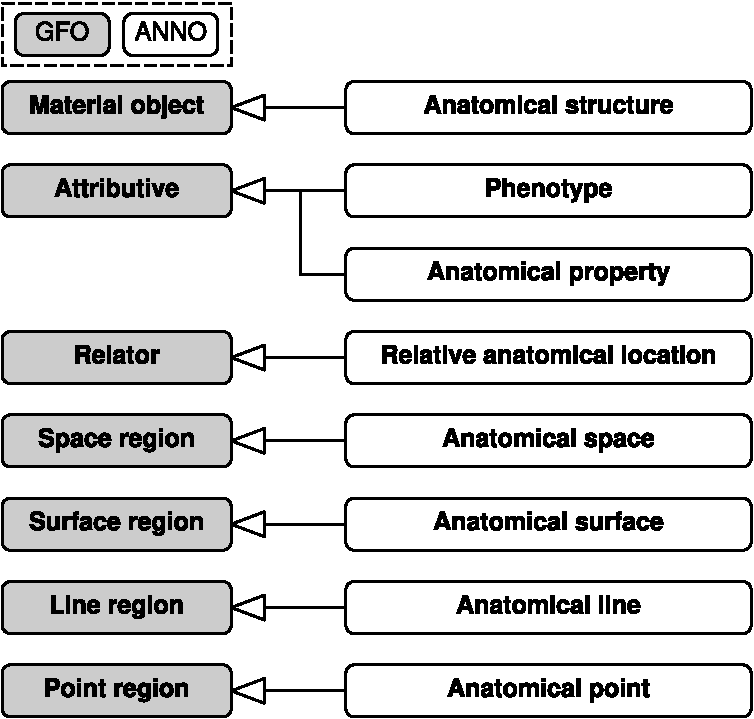
\includegraphics[width=0.6\textwidth]{img/gfo.pdf}
\caption{Integration of ANNO with the top-level GFO ontology.}\label{fig:gfo}
\end{figure}

% take care to prevent the problems noted by reviewer 1 in https://semantic-web-journal.net/content/modelling-digital-health-data-examode-ontology-histopathology
% TODO: ontology language, expressivity
% TODO: reuse of ontological entities
% TODO: clear validation mechanism
% TODO: top-level ontology?

\section{Description and Foundation of ANNOdc}\label{sec:core}
The core ontology development occurs in close collaboration between ontologists and anthropologists.
The objective is twofold: to adequately represent the most basic anatomical and anthropological entities and to keep the ontology relatively simple and compact.
This approach ensures that domain experts can easily handle the ontology and efficiently integrate it into the \aw{} software, see \cref{sec:aw}.

% Definition/Beschreibung der Kern-Konzepte/Module und -Relationen mit Beispielen, GFO-Einbettung
\begin{figure}[h]
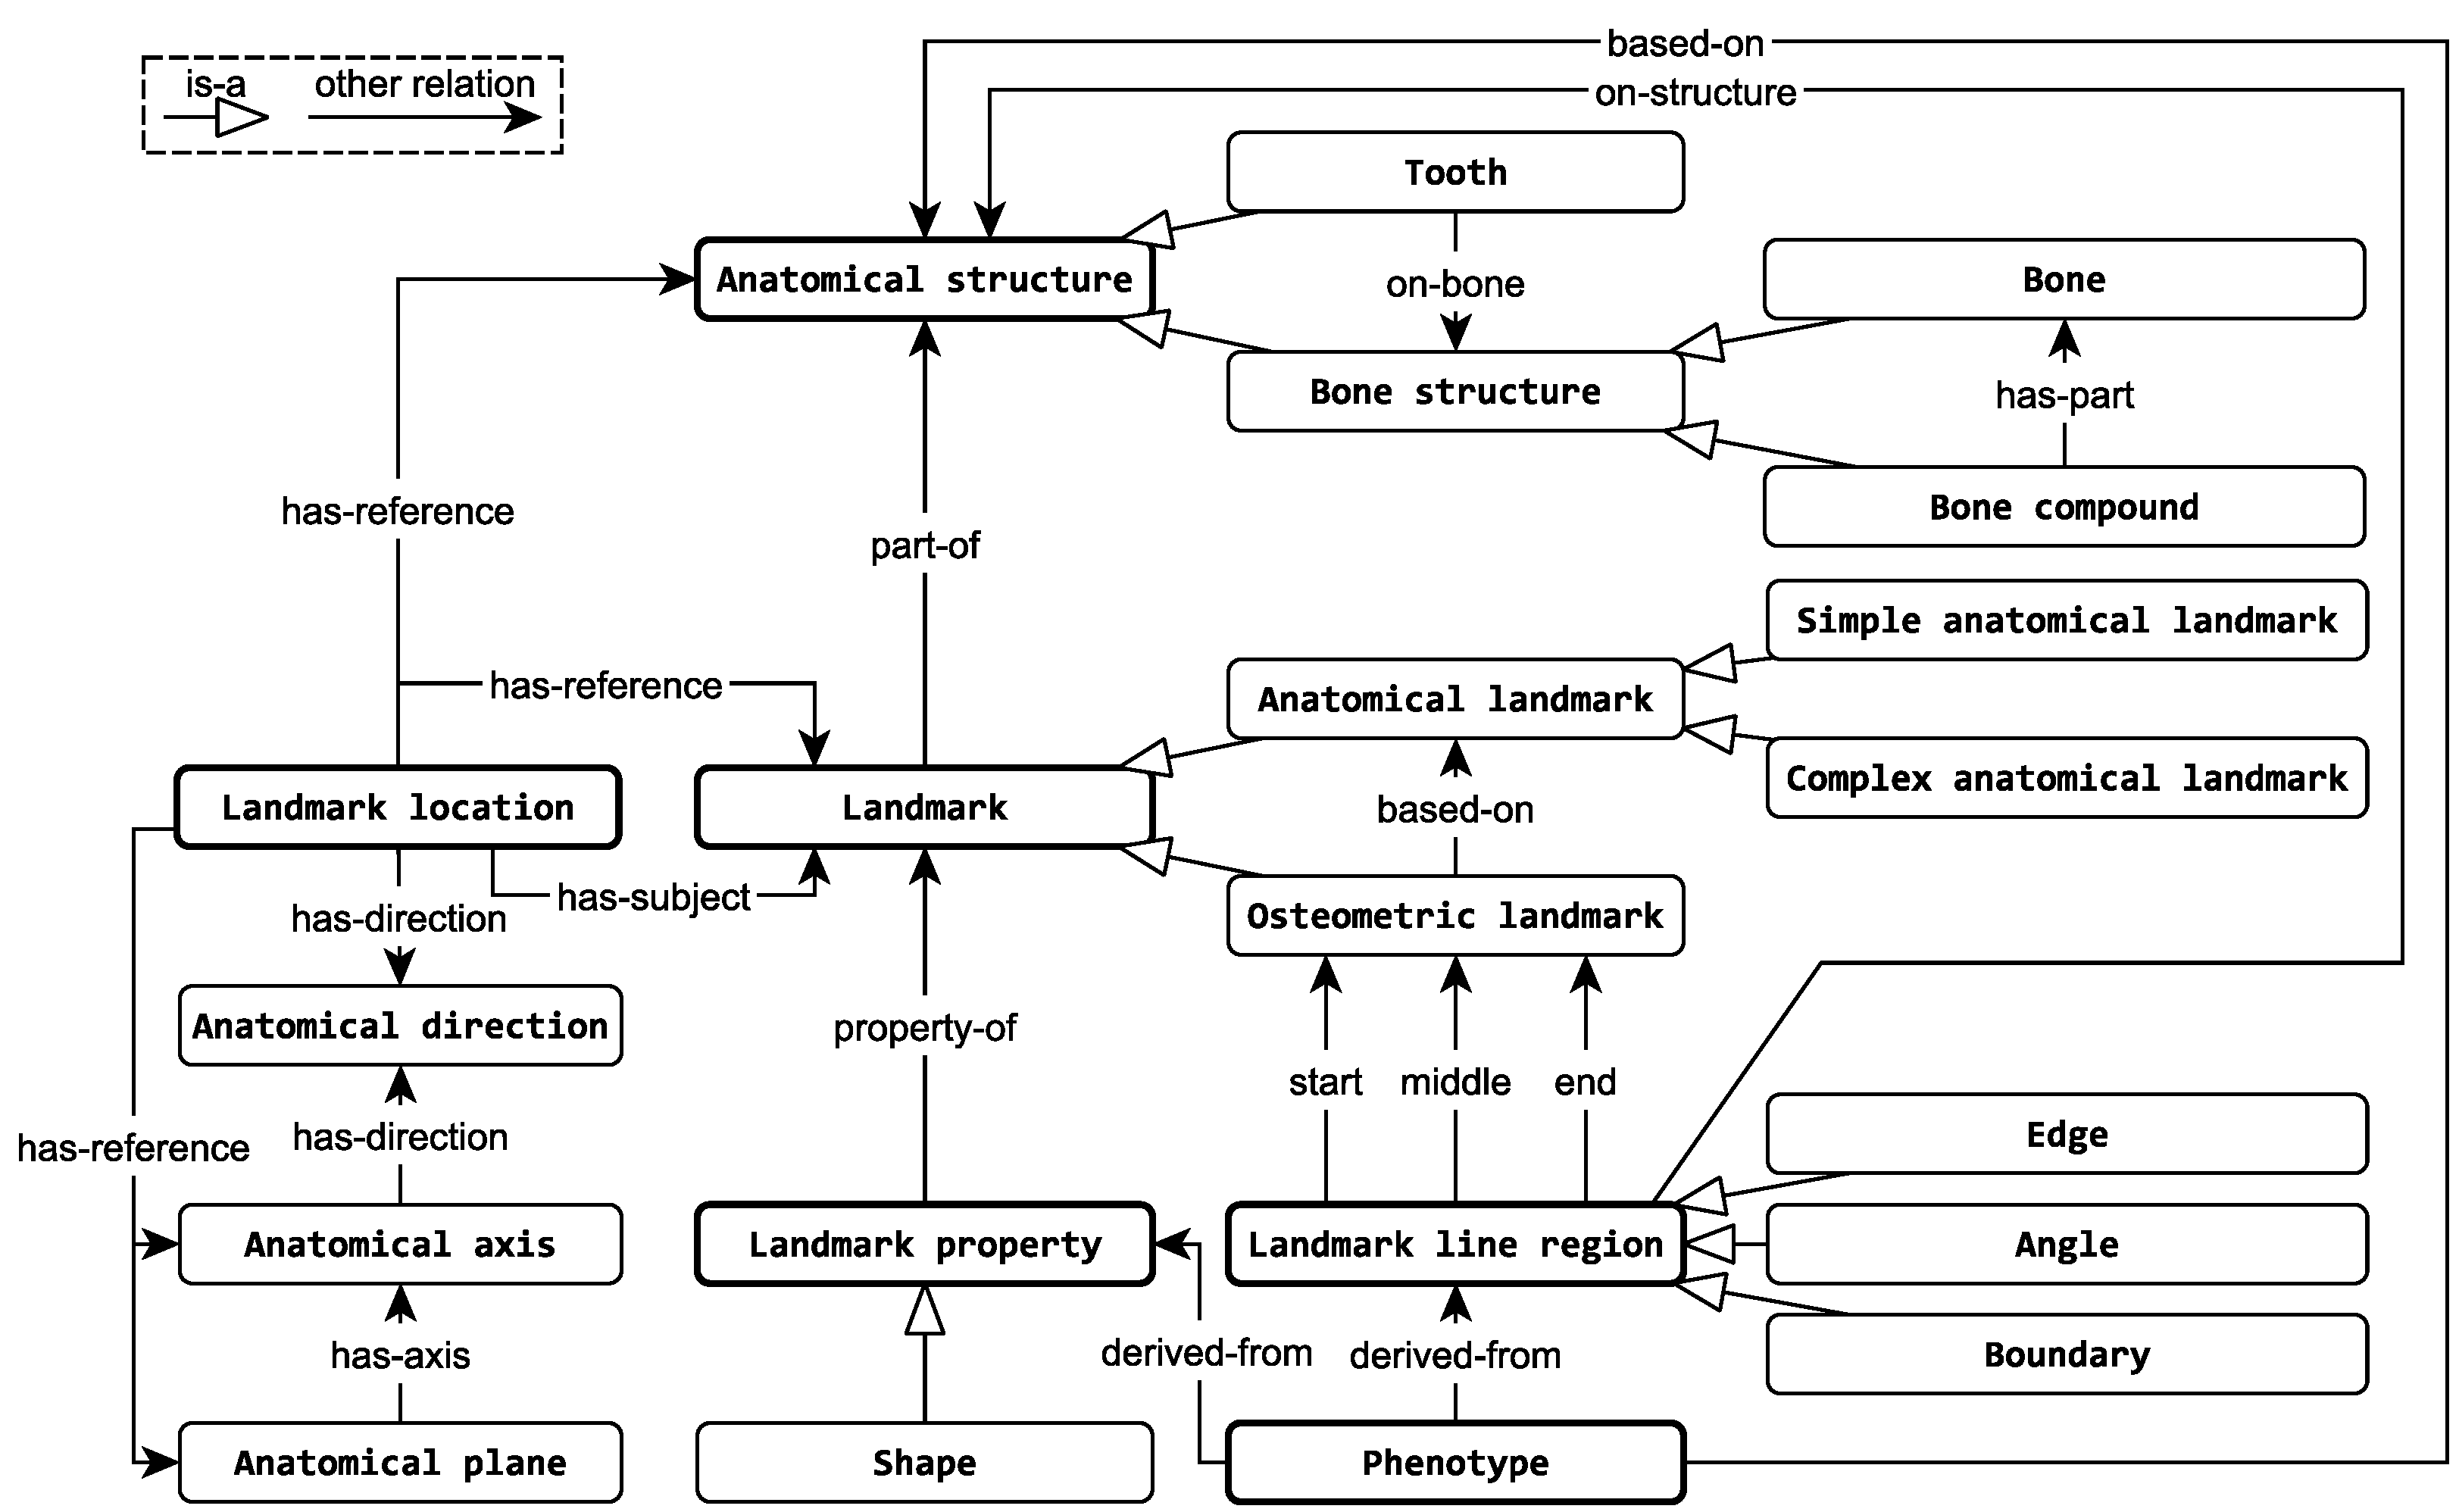
\includegraphics[width=\textwidth]{img/core.pdf}
\caption{The ANNOdc domain-core ontology.}\label{fig:core}
\end{figure}

\begin{table}[b]
  \centering
  \caption{Classes of ANNOdc along with exemplary ANNOds subclasses as well as interlinks to the FMA and the GFO top-level ontology.
  \textsuperscript{i}\anno{LO} is the line between \anno{Lambda} and \anno{Opisthion}, the \emph{occipital saggittal arc}.}
  \label{tab:core}
  \begin{tabulary}{\textwidth}{llLl}
    \toprule
	ANNOdc class					&ANNOds Examples				&FMA equivalent / ID						&GFO superclass	\\
	\midrule
	\anno{AnatomicalEntity}			&						&Physical anatomical entity \fma{61775}\\
	\anno{AnatomicalStructure}		&\anno{Skeleton}		&Material anatomical entity	\fma{67165}		&\gfo{MaterialObject}\\							
	\anno{SpatialAnatomicalEntity}	&						&immaterial anatomical entity \fma{67112}	&\gfo{SpaceEntity}\\
	\anno{AnatomicalSpace}			&						&											&\gfo{SpaceRegion}\\
	\anno{AnatomicalSurface}		&						&Anatomical surface \fma{24137}			&\gfo{SurfaceRegion}\\
	\anno{AnatomicalLine}			&\anno{LO}\textsuperscript{i}	&Anatomical line \fma{9657}	&\gfo{LineRegion}\\
	\anno{AnatomicalPoint}			&						&Anatomical point \fma{9658}							&\gfo{PointRegion}\\
	\anno{MeasurementPoint}			&\anno{Lambda}\\%, \anno{Ophistion}\\
	\anno{OrientationPoint}			&\anno{Orbitale}\\
	\anno{AnatomicalPlane}			&\anno{FrontalPlane}	&Anatomical plane \fma{242982}\\
	\anno{AnatomicalAxis}		 	&\anno{SagittalAxis}\\
	%\anno{Skeleton}					&						&Osseous skeleton \fma{23875}\\
	\anno{BoneStructure}\\
	\anno{Bone}						&\anno{Mandibula}				&Bone organ \fma{5018}\\
	\anno{BonePart}					&\anno{ArcusAlveolaris}	&Related to Segment of bone organ \fma{281808}, Zone of bone organ \fma{10483}\\
	\anno{BoneCompound}				&\anno{Cranium}				&Comparable to union of Skeletal system \fma{23881} and subdivision of skeletal system \fma{85544}\\
	\anno{ToothStructure}\\%			&\anno{DentesPermanentes}\\%		&Permanent teeth (\fma{75152}\\%; TA2ID:913)\\
	\anno{Tooth}					&\anno{DensCaninus}			&Tooth \fma{12516}\\
	\anno{ToothPart}\\%\fma{56481}; TA2ID:925\\
	\anno{Phenotype}				&\anno{SexGiles19671}			&											&\gfo{Attributive}\\
	\anno{AnatomicalProperty}		&						&													&\gfo{Attributive}\\
	%\anno{AnatomicalProperty}		&Shape (Degree of morphological expression)	&Anatomical relation, e.g., Has\_shape &\gfo{Attributive}\\
	\anno{RelativeAnatomicalLocation}&\anno{Sinister}	&Anatomical qualitative coordinate \fma{30346}	&\gfo{Relator}\\
	%\anno{RelativeAnatomicalLocation}&superior, lateral, medial, posterior	&Anatomical qualitative coordinate	&\gfo{Relator}\\
\bottomrule
\end{tabulary}
\end{table}

\subsection{Terminology for descriptive anatomy}

\begin{figure}
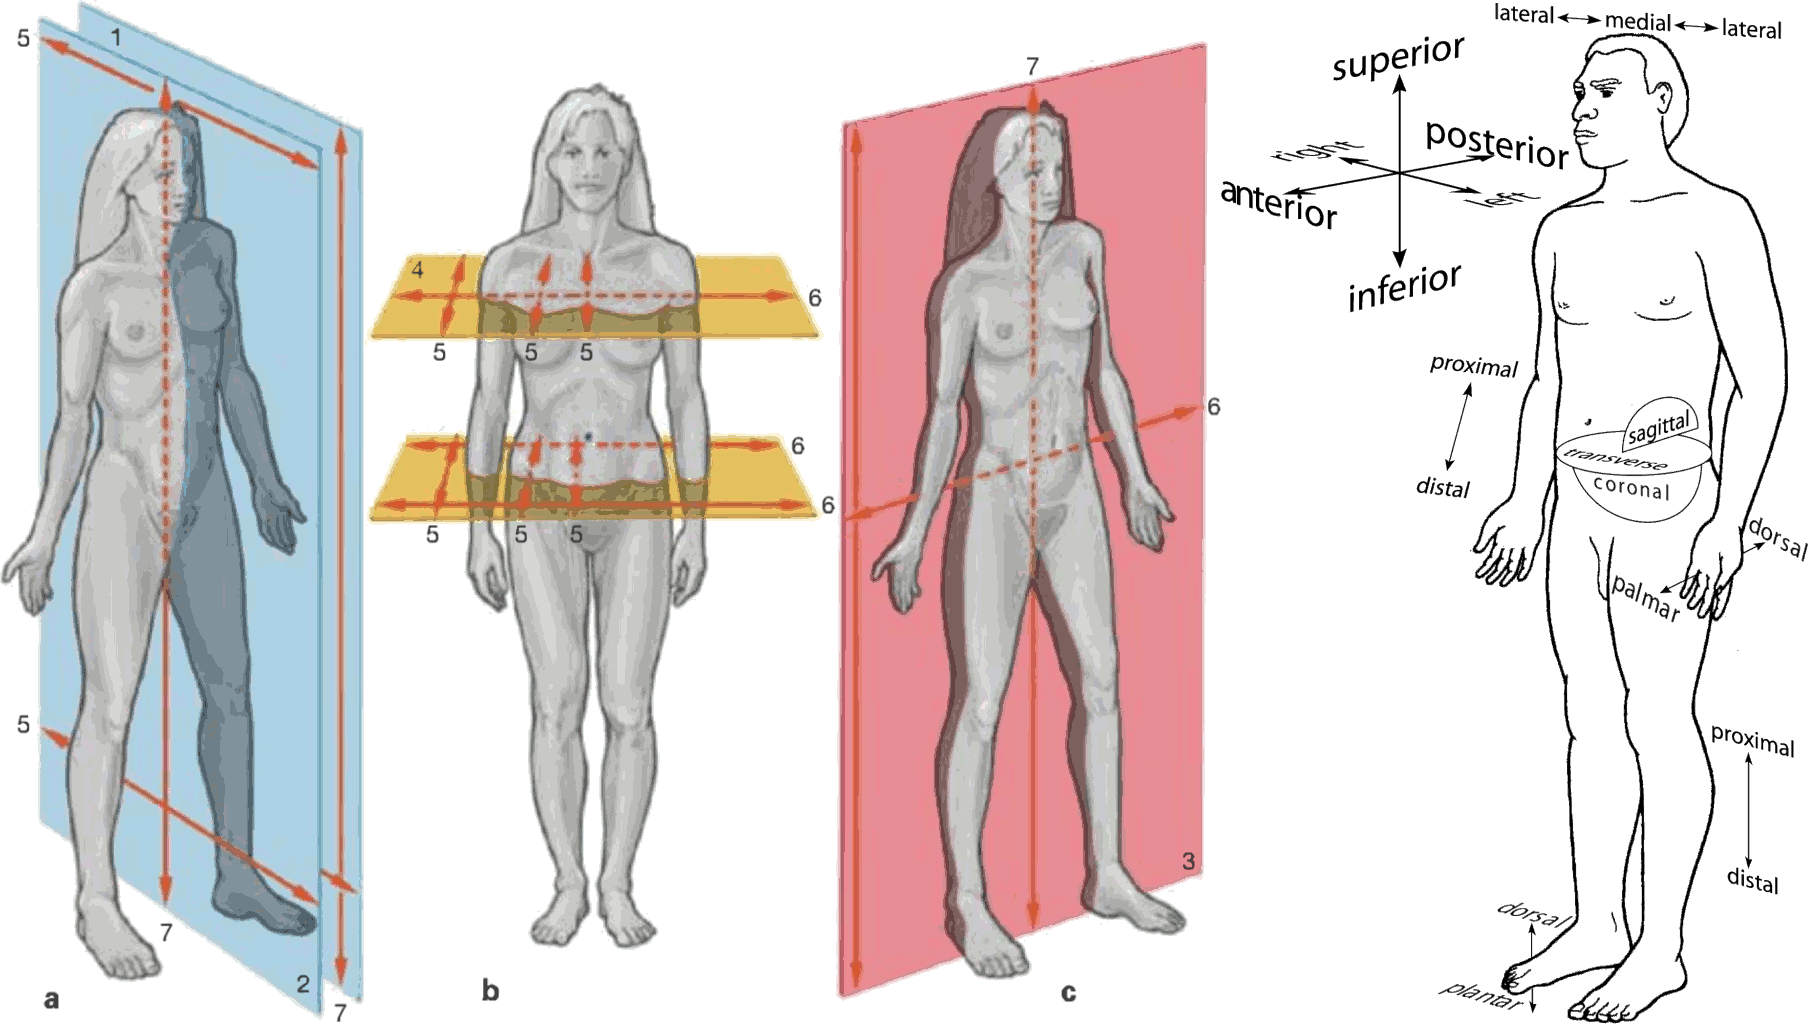
\includegraphics[width=\textwidth]{img/axisplanelocation.png}
\caption{Left: Anatomical Planes and Axes:
1 saggital plane,
2 midsaggital plane,
3 frontal plane,
4 transverse or horizontal plane,
5 saggital axis,
6 transverse axis,
7 longitudinal or vertical axis.
a: Planum sagittale (sagittal plane), includes sagittal and longitudinal axes; the midsagittal plane passes through the midline of the body,
b: Planum transversale (Transversal plane), includes transverse and sagittal axes,
c: Planum frontale (frontal plane): includes longitudinal and transverse axes.
Right: Anatomical relative location: directional terms used in anatomy and anthropology.
Modified figure based on \cite{allgemeineanatomieen,schemamann}.}
\label{fig:axisplane}
\end{figure}
%\FloatBarrier
The position of all anatomical entities is described in a standardized fashion using conceptual axes (a kind of anatomical line), planes (a kind of anatomical surface) as well as directions (relative anatomical locations).
Directions are relative to the body based on the standard anatomical position (\emph{positio anatomica} \aurl{ta2}{72}, \aurl{fma}{23132}).
It refers to standing upright, facing forward, palms and toes pointing forward, thumbs to the side, and observed from the perspective of the respective individual. %Quelle kommt noch
%
Although an infinite number of axes and planes can be defined within the human body, generally three principal axes and planes are used~\citep{prometheus}.
They are mutually perpendicular and provide the three spatial coordinates.
The three principle axes, shown in \cref{fig:axisplane} are:
\begin{itemize}
\item The longitudinal or vertical axis runs in the superior-inferior direction in an upright position, perpendicular to the ground.
It intersects with the frontal and sagittal planes.
\item The sagittal axis runs in the ventral-dorsal direction, from the front to the back surface of the body and vice versa.
It intersects with the sagittal and transverse planes.
\item The transverse or horizontal axis extends from left to right, intersecting with the frontal and transverse planes.
\end{itemize}

The three principal planes, depicted in \cref{fig:axisplane}, are:
\begin{itemize}
\item The sagittal plane, i.e all vertical planes parallel to the sagittal suture of the skull and running from anterior to posterior in the upright position.
The median (sagittal) plane divides the body into two symmetrical halves.
\item The frontal plane (= coronal plane) comprising all planes parallel to the forehead (frons) or the coronal suture of the skull, running vertically from one side of the body to the other in the upright position.
\item The transverse plane including all horizontal cross-sectional planes, relative to the upright position, dividing the body into cranial and caudal sections.
They run perpendicular to the longitudinal axis of the body.
\end{itemize}

Each one has two anatomical axes as boundaries in the sense of GFO, which allows boundaries to occur inside a structure and not necessarily at the extremities.
For example, the coronal (frontal) plane has the transversal (horizontal) and longitudinal (vertical) axes as boundaries.

An anatomical direction or relative anatomical location, as shown in \cref{fig:axisplane}, is the position of an anatomical entity (e.g., a bone structure) in relation to another anatomical entity (e.g., another bone, an axis, a plane or a point such as the center of the body).
Relative anatomical locations are classified according to the anatomical terms of location (e.g., cranial or superior = \enquote{towards the end of the skull}, dexter = \enquote{right} or distal = \enquote{in direction towards the end of a limb}).
For example, the Glabella is located laterally to both Arcus superciliaris (Arcus superciliaris sinister und Arcus superciliaris dexter).
A relative anatomical location can be considered as an individual relation between two anatomical entities (target entity and reference entity) and can therefore be modeled using a GFO relator.
Relators are composed of roles (in our case target and reference) and have the power to relate arbitrary entities (in our case, anatomical entities)~\citep{gfocategory}.


\subsection{Anatomical entity}
An anatomical entity is either an anatomical (material) structure or a spatial anatomical entity, such as \anno{Cranium} or \anno{FrontalPlane}.

\subsection{Anatomical structure}
An anatomical structure refers to any anatomical division or material anatomical entity.
ANNO describes three kinds of anatomical structures: tooth structures (teeth and teeth parts), bone structures (single bones, bone parts and bone compounds), as well as the complete skeleton.
The GFO defines a material object \aurl{gfo}{MaterialObject} as a solid concrete entity that belongs to the material region of the world, has mass, consists of matter and occupies space~\citep{gfospace}.
Accordingly, we define anno:AnatomicalStructure as a gfo:MaterialObject in the anthropological context.
The closest equivalent in the FMA is the \emph{Material anatomical entity} \aurl{fma}{67165}, the subclass of \emph{Physical anatomical entity} \aurl{fma}{61775} that has mass.

\subsection{Skeleton}
The largest or most comprehensive skeletal anatomical structure, the human skeleton, is the framework composed of all the bones and teeth of a human being.
The TA~\citep{ta2} equates the skeleton with the \enquote{Systema skeletale (skeletal system)}, which refers to the passive part of the musculoskeletal system, including the articulated bony skeleton with teeth, as well as cartilage, ligaments, and other joints.
ANNO does not adopt this equivalence, and \enquote{Skeleton } here refers to the entirety of a human's bones and teeth.
However, since teeth constitute their own tissue, they are treated separately, allowing all other components of the skeletal system, such as cartilage or ligaments (as tissues) or joints (e.g. as specific aspects), to be integrated and referenced separately in ANNO.
The anthropologically meaningful distinction between \enquote{Skeleton} and \enquote{Systema skeletale} can be maintained, while still referencing both within the TA concept.

\subsection{Tooth structure}
Tooth structures comprise teeth and their parts.
A human tooth is an individual unit of the human dentition (synonymous for the teeth as a whole).
Teeth are part of the skeleton, yet they are characterized by their own distinctive tissue and thus treated separately from bones.
Teeth, such as the Dens caninus (canine tooth) are located on bone structures.
The FMA has the equivalent class \enquote{Tooth} \aurl{fma}{12516}.
A tooth part is any portion of a tooth.
They are not included in the initial scope of the ontology, but they are one of the aspects by which it can be expanded.

\subsection{Bone structure}
Bone structures comprise all possible parts of the human skeleton, which are individual bones, bone parts, bone compounds as well as the complete skeleton excluding the teeth.
The FMA does not have a common superclass for those parts but instead mounts them in different parts of its hierarchy.

A bone or bone element is a single self-contained bony skeletal entity.
Bones, such as Mandibula (Mandible) and Os occipitale (Occipital Bone) are individual bone organs.
FMA does have a \enquote{Bone} class (\aurl{fma}{30317}) but that only has a single subclass \enquote{Skull bone} (\aurl{fma}{30317}).
Instead, \enquote{Bone organ} (\aurl{fma}{5018}) is the equivalent class.

A bone compound is a section of the skeleton combining multiple bones or bone parts together, depending on the classification system chosen.
This allows for the representation of any partonomy that need not necessarily be compatible with one another.
Bone compounds, such as the Cranium (skull bone) consist of further bone compounds, individual bones (which in turn consist of bone parts) and bone parts.
The FMA does not have a single equivalent class, but it is similar to the union of \enquote{Skeletal system} (\aurl{fma}{23881}) and \enquote{Subdivision of skeletal system} (\aurl{fma}{85544}).
On the skeletal level, bone parts comprise any piece or portion of a bone.
An anatomical landmark is any distinct structure on a bone.
In ANNO, it is also referred to as a bone part.


\subsection{Spatial anatomical entity}
An anatomical entity without mass is classified as a spatial anatomical entity, which is either an anatomical space (three-dimensional), an anatomical surface (two-dimensional), an anatomical line (one-dimensional) or an anatomical point (zero-dimensional).
It is equivalent to the FMA \enquote{Immaterial anatomical entity} (\aurl{fma}{67112}).

An anatomical space is a space region (three-dimensional) occupied by an anatomical structure.
An anatomical surface is a boundary (two-dimensional) of an anatomical space.

An anatomical point (or osteometric landmark) is any immaterial, conceptual point that marks a location on a bone, either to create measurements (anatomical lines) or locate other anatomical points, e.g. by aligning the bone in specific planes for a measurement.
The former serve as measurement points, the latter - relevant to the measurement procedure as orientation points.
An anatomical point is thus a boundary (zero-dimensional) of an anatomical line.

An anatomical line is a conceptual, immaterial line on a bone passing between at least two measurement points that, in the form of distances, circumferences or angles is used to collect measurements representing aspects of a bone's dimensions.
An anatomical line is a boundary (one-dimensional) of an anatomical surface.
Anatomical lines can connect or pass through anatomical entities (e.g., an edge between two or an angle between three anatomical entities).
The length of the line or the angle degree can be measured and used in functions to infer individual phenotypes.% [Verweis zu Phenotype section].

\subsection{Phenotype}
\begin{figure}[h]
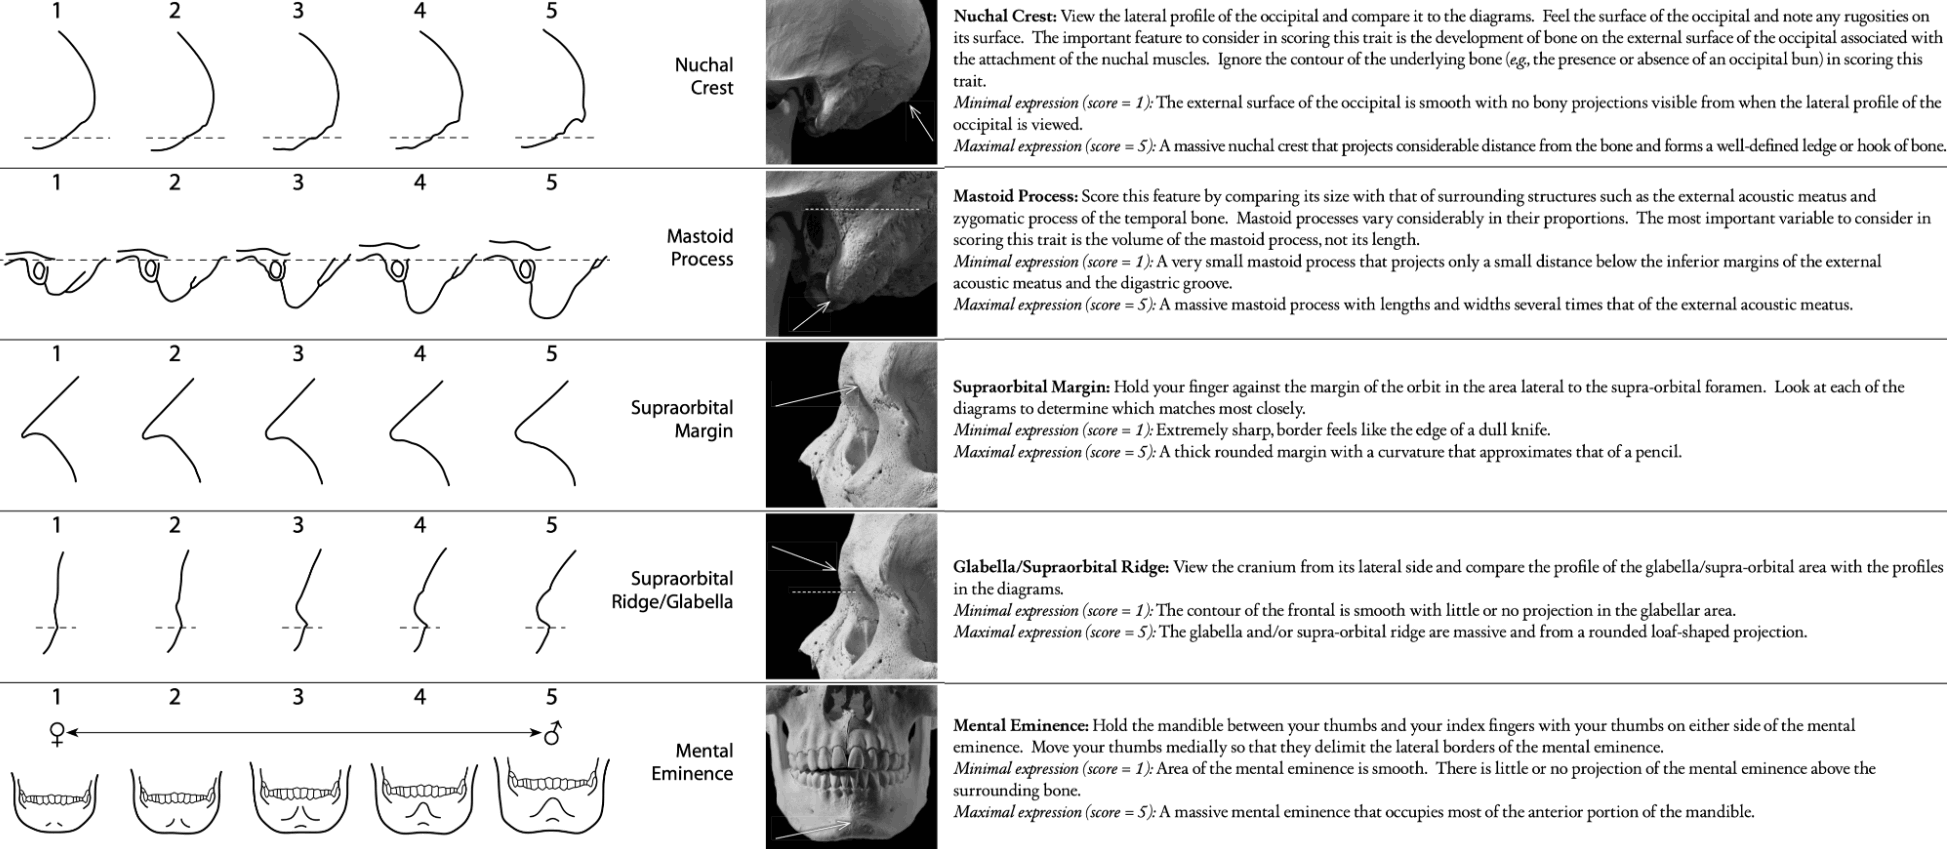
\includegraphics[width=\textwidth]{img/phenotype.png}
\caption{
Exemplary assessment of anatomical properties for the derivation of the phenotype sex, where five cranial bone parts are evaluated for their level of morphological expression.
% yes, walker method is published in buikstra
Method after Walker~\cite{datacollection}.
Image taken unmodified from \cite{datacollection}.
}\label{fig:phenotype}
\end{figure}


Usually, a phenotype is considered as a (combination of) bodily feature(s) or observable characteristic(s) of an organism, such as sex, body height or body weight~\citep{ontologicaltreatment,phenomes,interoperability}.
Since phenotypes are individual properties, they can be considered as attributives in the GFO sense.
The phenotype notion has also been analyzed in detail within the framework of the Core Ontology of Phenotypes~\citep{ontologicalrepresentation}.

In the case of ANNO, the phenotype can be derived using functions comprising obtained measurements.
Discriminant functions, e.g. based on the Cranium, allow for the assignment to sex while estimation of stature is attained by using linear regressions, e.g. based on Femur or Tibia length measurements.
RDF is not optimized for mathematical formulas so we model those as literals.

% ć in Vodanović cannot be displayed without font package and I don't know if the journal allows a different font
As an example, the discriminant function no. 6 developed by Vodanovic uses the measurement of the angus mandibulae to assign sex, thus deriving a phenotype.
For the left side it is given as:
\[
0.17 \cdot [\text{ppam sinistrum-go sinistrum-paim sinistrum}] - 20.43
\]
The right side is calculated analogously using (ppam dexterum-go dexterum-paim dexterum).
%\[
%\text{For the right side: } ([\text{ppam dexterum-go dexterum-paim dexterum}] \times 0.17) - 20.43
%\]
The threshold or sectioning point is given at 0.2, meaning that if the result is greater than this value, then sex is assigned to male, if it is lower it is assigned to female.

\subsection{Anatomical property}
An anatomical property is a characteristic (e.g., shape) of an anatomical structure.
Anatomical properties are considered as attributes or qualities in GFO~\citep{gfoarchitecture}.
These are dependent individuals that characterise other individuals (in our case, anatomical structures).

Other than by means of osteometry using measurements and functions, an anatomical landmark's morphology can be used to examine anthropological aspects or phenotypes such as age or sex.
For instance, assessment of the degree of an anatomical landmark's morphological expression (the anatomical property in this case) offers information about the sex of the remains of the individual being examined.
While the morphological examination was not within the scope of the project, it was nonetheless ensured that future extension in this respect is possible.

\section{Development of ANNOds}\label{sec:domain}

\begin{figure}[h!t]
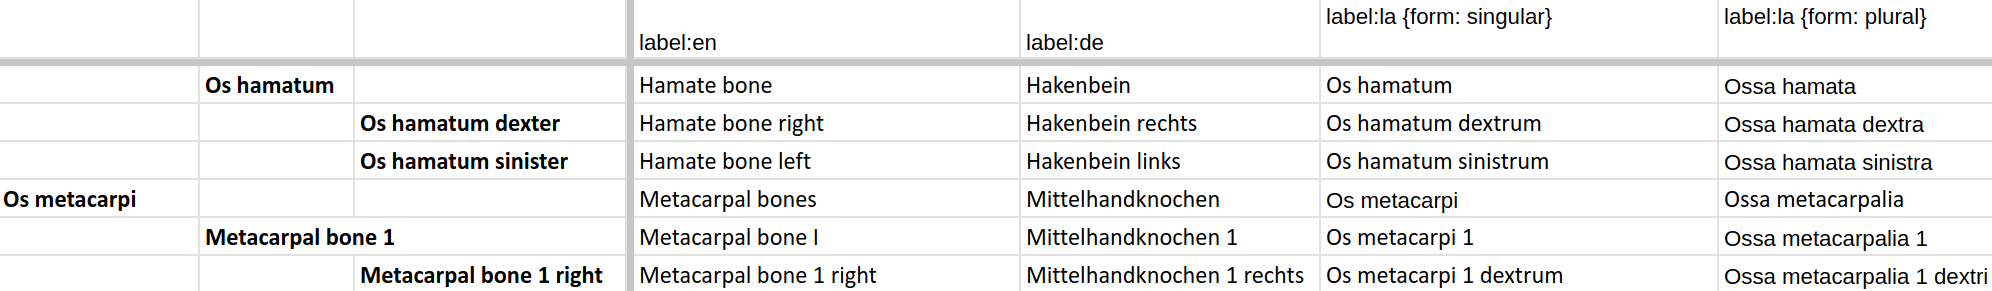
\includegraphics[width=\textwidth]{img/smog.png}
\caption{Excerpt of the spreadsheet-based input template used by the anthropologists.}\label{fig:smog}
\end{figure}

\begin{figure}
\centering
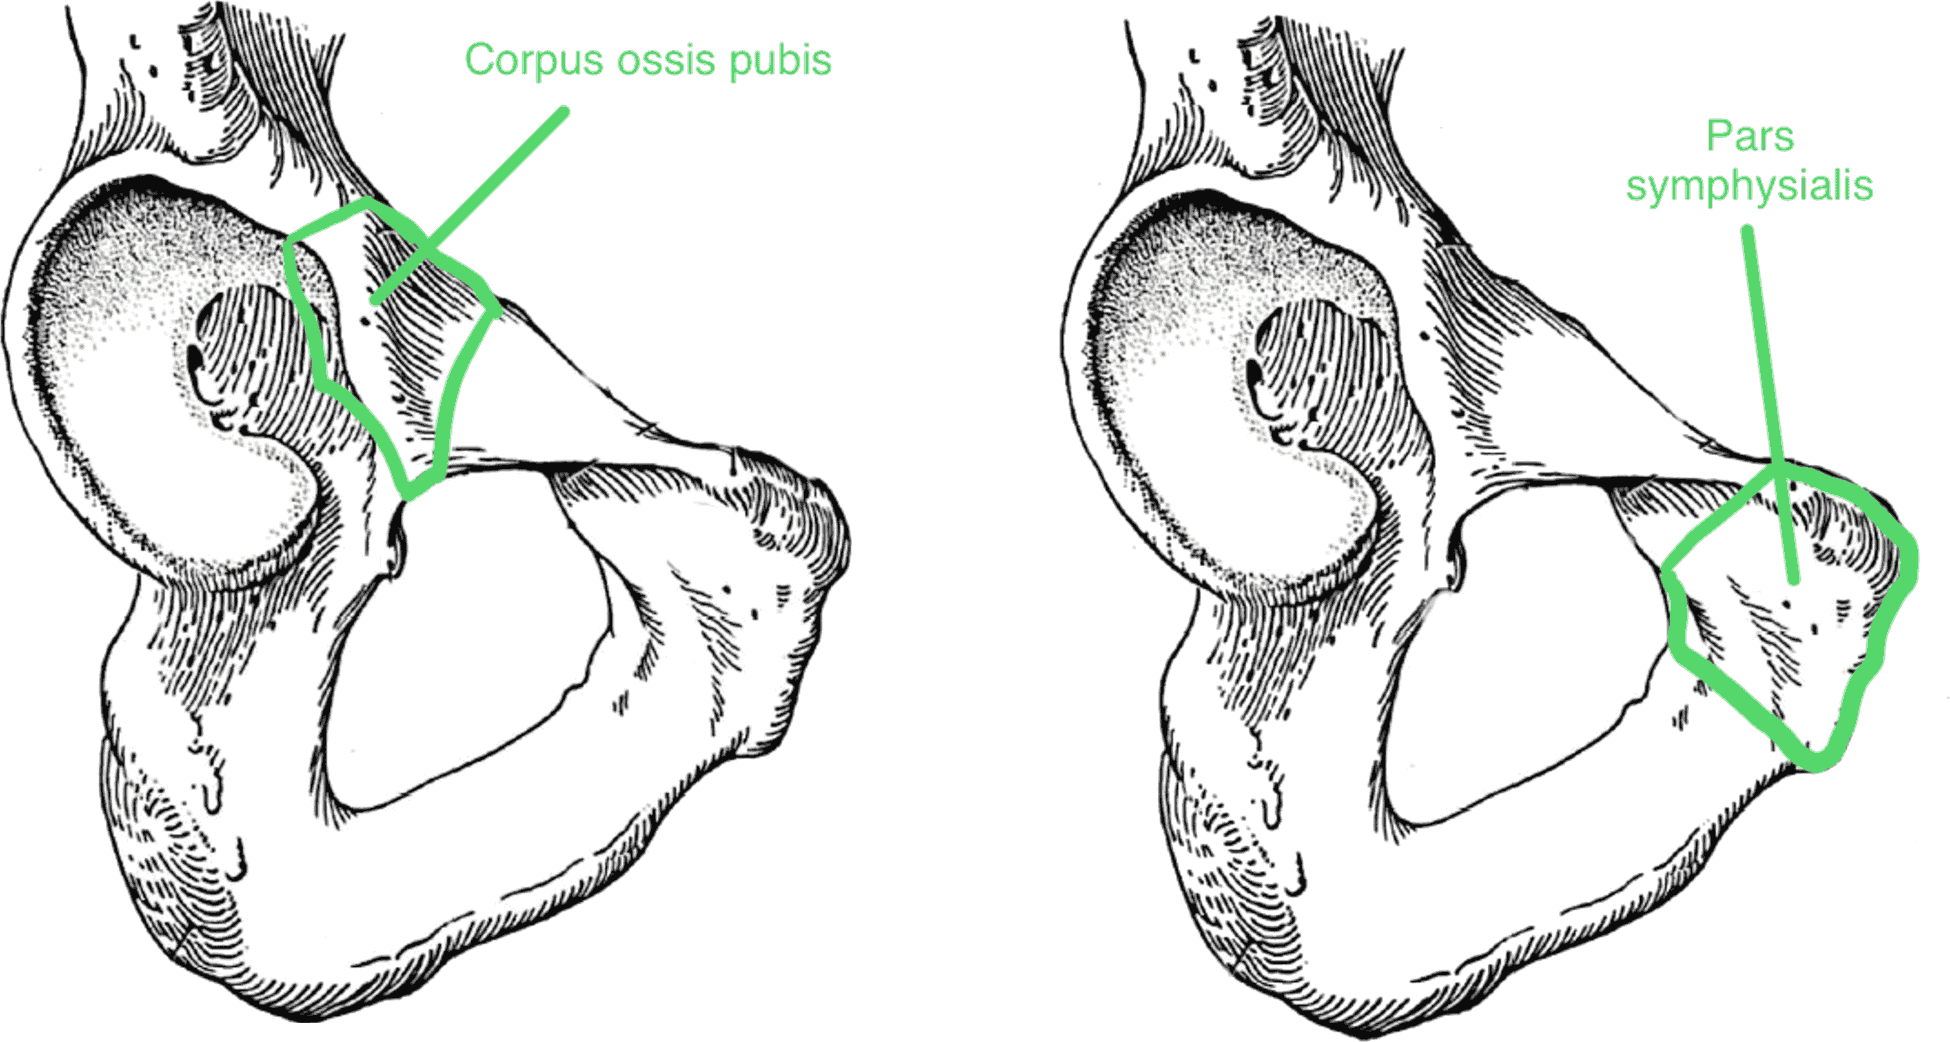
\includegraphics[width=0.6\textwidth]{img/corpus_ossis_pubis.png}
\caption{}\label{fig:corpus_ossis_pubis}
\end{figure}

While ANNOdc is created by the ontologists in consultation with the domain experts, ANNOds is developed by the domain experts themselves.
For this purpose they were provided with a spreadsheet-based SMOG~\citep{smog} template by the ontologists, see \cref{fig:smog}, eliminating the requirement of having a background in RDF and ontologies.
The template is based on the structure of ANNOdc, so that the entered data is compliant with it: The ANNOds classes are subclasses of the ANNOdc classes (see \cref{tab:core}) and properties (see \cref{fig:core}) from ANNOdc are used.
The spreadsheet is transformed to an OWL 2 ontology consisting of a taxonomy, annotations and some simple axioms on the basis of property restrictions.
This approach ensures intuitive and unimpeded data input and a valid end result.
The primary focus is on the design of ANNO's ontological architecture and the conception of the process for creating the content, as well as on the integration into the Applied University of Mittweida's in-house software AnthroWorks3D.

In addition, the objective is to initiate the process of data entry, encompassing selected bones of the skeleton.
%
%\textbf{UNFINISHED DRAFT SECTION, TO BE HEAVILY REWORKED AND CUT}
%\subsections{General considerations}
%All landmarks are annotated with their name in singular and plural form, reference bone, synonyms, textual and visual definition, FMA and TA ID, and sources.
%
%Anatomical Landmarks (Bone Parts)  (Selection Criteria, scope and process,  properties) 
%Osteometric Landmarks (Anatomical Points) 
%Measurements (Anatomical line)  
%Relevant spatial anatomical objects (e.g., lines) used for phenotype determination functions Measurements were defined in terms of anatomical points/objects that bound them: consist of references to sections, the start point, midpoint, and end, and short definitions.
%Phenotypes 
%Development of the ontology is based on the following selection criteria:
%The selection criteria are as follows:
Given the overwhelming number of bone parts present in the cranium, the initial selection was narrowed down to a selection of representative and relevant parts.
Overall, however, the aim is to include those that are of anthropological relevance, i.e. that contribute to navigation, localization, and identification on the bone.
Those structures included in the definitions of others were also to be defined.
For bones that lie on the median sagittal plane (e.g., mandible or sternum), bilateral landmarks are defined, each with a side reference.
For osteometric landmarks, all those already established in the core literature are to be used.
Furthermore, those that are relevant for meaningful measurement distances and can be annotated in \aw{} should be used.
For the measurement distances, those should be selected that are established in the majority of the core literature as well as necessary for discriminant functions and functions for estimating height and weight.
%In addition, it also had to be integrable into \aw{}.
The functions chosen were those with diagnostic value.
These were discriminant functions for sex determination and regression functions for body height and body weight estimation.

%\subsection{Process for creating definitions and measurements}
For the definitions and measurements, a representative minimum amount of anthropological and anatomical English- and mostly German-language literature was compared in order to develop the definitions from their information.
Notably, Latin or latinized ancient Greek terms often missing in the English literature and the FMA were included.
%The FMA also contains only English terms.
%For this reason, these were also searched with their synonyms.
Overall, the name of the structure, measurement or point is noted in Latin in singular and plural forms, English, German, synonyms in all three languages, the FMA and TA ID, and any information on function and delineation.
This requires a positional description, such as the Punctum superioris capitis femoris as the superior located point of the Caput femoris.
%The examination of the Latin grammar was relevant for this.
For the measurements, in addition to the name of the measurement, the type (e.g., distance measurement) and the measurement instrument were also recorded.
The subsequent visual definitions were made in the different anatomical views marking the area of the anatomical structures and the position of the anatomical points.

%\subsection{Functions}
The functions are divided into discriminant functions for sex determination and regress functions for body height.
The sex of a specific individual within a population may be estimated using a function on skeletal measurements that is specific or similar to this population.
Based on a threshold value, skeletons are classified into male, probably male, indifferent, probably female, and female.
The exact number of categories may vary depending on the particular method used.
ANNOds covers functions for at least one European, African, American, and Asian ethnicity or population.
%Names are assigned by the number included in each study, the authors, and the year of publication.
%In addition, the function, reference population, aspect (e.g., discriminant function), and sample size with division by gender are noted.
%For the discriminant functions, the thresholds of sex assignment, classification accuracy, and misclassification are important; for the regression functions, the error interval is important.
%
%While there are many textual sources of anthropological systematisation, they do not agree in all aspects and there is not a single, formally described, standard.
%ANNO links to concepts of the FMA when they exist, but structures them in a different way.
%
%\subsection{Sex determination}
% auto translated from the project report, use as basis:
%
%\subsection{Regress functions}
%Regress functions for body height and body weight estimation.
%Names were assigned by the number included in each study, the authors, and the year of publication.
%In addition, the function, reference population, aspect (e.g., discriminant function), and sample size with division by gender were noted.
%In addition, for the discriminant functions, the thresholds of sex assignment, classification accuracy, and misclassification were important; for the regression functions, the error interval was important.
%
%Standardised description of position 
%In addition to the conception and development of the ontology as well as of definition, data input was initiated as content of Cranium including the Mandibula as well as the teeth of the was entered. Entries can be added directly to the OWL-File using Protégé or they can continue to be entered directly into the spreadsheet. In the latter case, the OWL file can be generated with a custom OWL generator.

\section{Use Case: Integration into \aw{}}\label{sec:aw}

\todo{
Import der Ontologiedaten in Anwendung in Form von JSON
Anpassung der bisherigen Anwendungsstruktur an Attribute der Ontologie
Zuordnung von Objekten (Markierungen, Messungen) in Anwendung zu Objekten der Ontologie
Import und (teil-)automatisierte Berechnung der Diskriminanzfunktionen (bspw. Geschlechterbestimmung)
}

\begin{figure}[h]
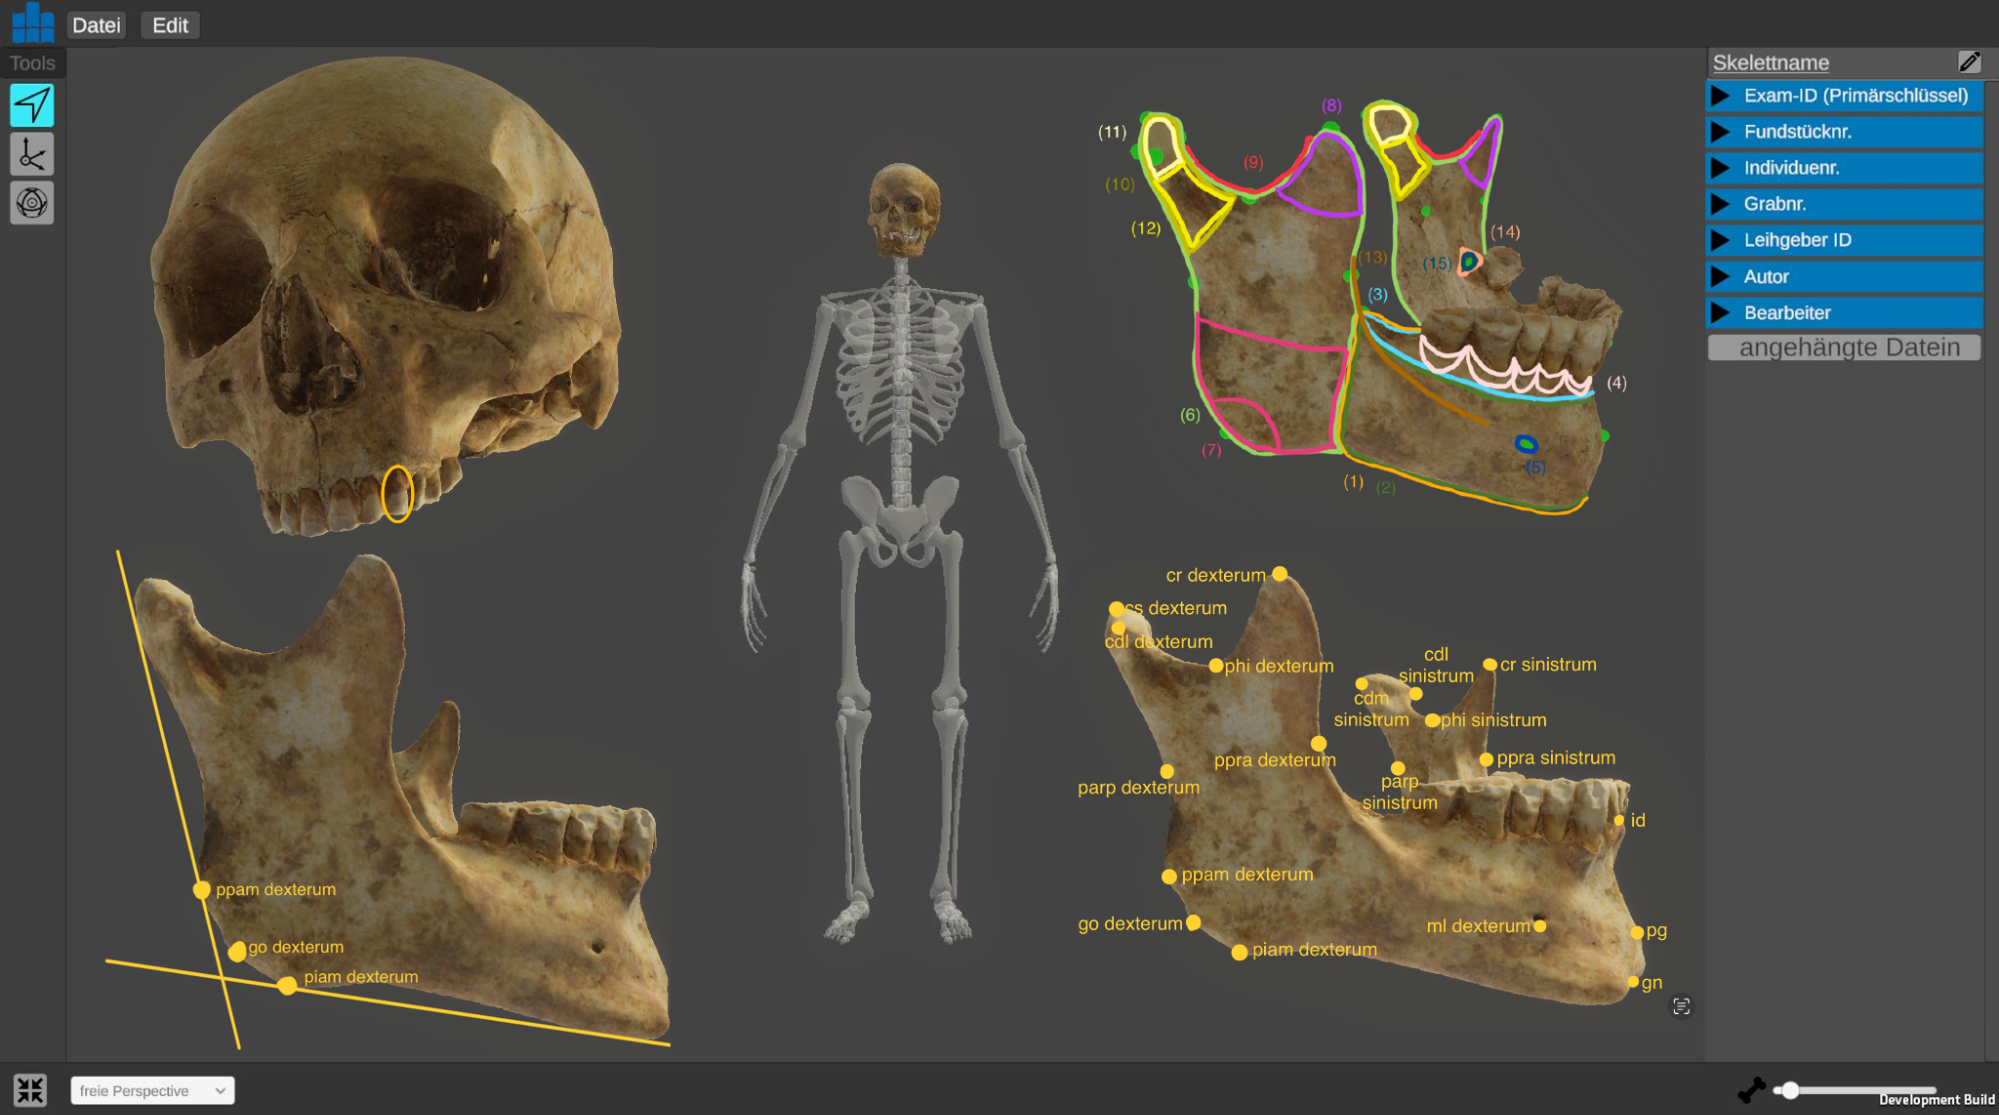
\includegraphics[width=\textwidth]{img/aw3d.png}
%\caption{3D model of a Cranium (skull) inserted into a placeholder skeleton in \aw{} depicting examples of various ANNOdc classes.}
\caption{
Collage of different views in \aw{} of a 3D model of a \emph{cranium} (skull) inserted into a placeholder skeleton (source:~\cite{aw3dcidoc}).
The cranium is a bone compound consisting of 29 bone elements.
One of them, the \emph{mandibula} (mandible), is flexibly connected to the rest of the skull by the mandibular joint.
In the top right, various bone parts on the Mandibula are visually emphasized, with part 14 representing the angulus mandibulae (mandibular angle).
In the top left, the \emph{dens caninus maxillaris dexter} (right maxillary secondary canine tooth), a tooth structure, is highlighted within a circle.
The tooth cusp is a part of the tooth.
It refers to the projection that divides the occlusal surface of most of the teeth, with the exception of the incisors.
At the bottom right, anatomical points (osteometric landmarks) of the right lateral side of the \emph{mandibula} are depicted.
The \emph{gonion dextrum} (right gonion; \emph{gonion dextrum}, abbreviated as \emph{go dextrum}, depicted alternative spelling of dextrum: dexterum) forms part of an anatomical line measuring the \emph{angulus mandibulae},
as shown in the bottom left.
Skeletal material courtesy of Dr. Birgit Grosskopf, Department of Historical Anthropology and Human Ecology, University of Göttingen.
}
\label{fig:aw}
\end{figure}

%\textbf{UNFINISHED DRAFT SECTION}

\aw{}, see \cref{fig:aw}, is a tool that combines user-friendly techniques of photogrammetry with insights from user experience research and knowledge from game development and offers a procedure to create 3D skeletal models serving as  digital twins  which can subsequently be examined virtually.
This facilitates anthropological work to be location-independent and parallel without exercising wear and tear on the skeletal material.
The examination can be performed as often as desired, even if the skeletal individuals or collections are not available at the institute or have already been reburied.
%
We use our ontological architecture (top level ontology, domain core ontology, domain specific ontology) to integrate ANNO into \aw{} based on the three-ontology method~\cite{threeontologymethod}.
%This method, as outlined in~\cite{threeontologymethod}, aided us in designing a tool for annotating human skeletons and identifying phenotypes. 
%We use ANNOdc as the Task Ontology and ANNOds as the Domain Ontology.
One of the advantages of the three-ontology method is that the software only needs to implement access to the entities (classes and properties) of ANNOdc ontology, whereas the classes of ANNOds are processed dynamically.
%\aw{} leverages ANNOdc as an interface to dynamically access the entities of the ANNOds, such as listing all subclasses of a specific class like \aurl{anno}{Bone}, as explained in \cref{sec:aw}.
%
\iffalse
It also draws its advantage when space is limited.
Thus, it requires only three SLR cameras, sufficient exposure and a computer.
The examination proceeds as follows: After photogrammetry is done and the 3D model is created, the objects are imported into the software and calibrated.
For calibration, there is an individual placeholder for each bone, which must first be selected.
Then the calibrated digital twin is placed in a placeholder skeleton.
Annotations can be made in the detailed view of each bone.
Point, line and area markings are available for selection.
Furthermore, it is possible to make measurements.
You can choose between distance, angle and circumference measurements.
After marking or measurement, an identification number is assigned to each one.
There is also a documentation about the time of the annotation as well as the name of the editor.
The marking or measurement can be classified according to certain categories (e.g. anatomical variation).
In addition, annotations are possible in a text field.
The annotations can be edited at any time afterwards, and the date of editing is recorded together with the author.
The annotations are subsequently displayed in different colors, so that overlaps can be kept apart.
A special feature of the software is the automation of measurements.
The program automatically sets pins for osteometric landmarks in a template view.
The person using the program can move these as desired.
The pins displayed have different color shades.
These differ depending on the relevance.
If the osteometric landmark is present in many measurement sections, its relevance increases and the pin appears darker.
After the pins have been roughly set, they can be refined using various views.
In the views, the individual osteometric landmarks are visible from different views, so that a fine adjustment can be made.
This is followed by the automatic measurement.
The individual values for each measurement section can be downloaded as a CSV file.
In addition, it is now possible to perform sex determinations using discriminant functions.
For this purpose, the required measurement sections can be selected.
The results are only visible in one display.
The automation allows a time saving, whereby more bones or skeletons can be examined in a shorter time.
Advantages over the previous approach are:

ontology-oriented generation of placeholders/containers for objects to be imported
variable properties for different bone elements and bone types
hierarchy for orientation within an examination project according to the ontology tree
categorization of measurements and markers according to specifications from the ontology
generation of input forms based on the specified properties and bone types
automatic generation of measurements
\fi

%\subsection{}\label{s1.1}
\section{Conclusion and Future Work}
% "desirablility" add source e.g. https://fipat.library.dal.ca/wp-content/uploads/2021/08/FIPAT-TA2-Part-2.pdf

By contributing systematic, standardized and clear definitions for (material and spatial) anatomical entities regarding the human skeleton as well as anthropological aspects such as the derivation of phenotypes, ANNO formalizes knowledge in the fields of anatomy and anthropology.
It encompasses all the essential elements for the routine use of anatomical terms in daily anthropological practice.
Integrating the ontology into AW3D enables its immediate application in anthropological analysis.

The ontology is interlinked with the TA and FMA and provides transparency by including all sources used to generate its content.
Moreover, it provides a method for conceptualizing the ontology and generating its content.
The ontology replaces an old, hard-coded format in \aw{}, which saves development time, separates annotation file compatibility from software versions, eases annotation through hierarchical browsing and improves interoperability and customization.
Also, ANNO comes with extensive documentation of the process and available resources.
Hence, foundations have been laid for its use and further development and management.

Navigating through plenty of options for designing an ontology makes consistency challenging to achieve.
As documented in the TA~\citep[part II]{ta2}, the choices frequently reflect the preference of a party having something included or named or structured in a certain way because it is considered relevant by a particular party.
ANNO represents a specialized ontology that builds upon existing ontologies such as FMA and TA.
However, meeting the diverse needs of the field and interdisciplinary requirements can only be accomplished through an ongoing, gradual process over time.

While ANNO serves as a foundation for describing anatomical terms, additional work is required to comprehensively cover the anthropological domain.
For instance, it only covers standardized normal adult anatomy.
Moreover, in order to remain permanently suitable for practical usage, the ontology must be continuously reviewed, updated, enriched or adapted to further needs.
Moreover, ANNO presents all necessary prerequisites to being extended to the other aspects of anthropological work with human skeletal remains.

Apart from continuing data entry, future work may involve the inclusion of other anthropologically relevant properties such as those that capture the morphology of the human skeleton and contribute to deriving phenotypes such as sex, age and developmental aspects, pathologies or ancestry.
In addition, tooth parts, deciduous teeth as well as anatomical variants could be added in the future.

Regarding skeletal anatomy, the representation of preservation status through the ontology would be of great use for anthropological work.
Furthermore, anatomical terms describing aspects of bone morphology or function, such as the Latin word \enquote{processus} which appear numerous times as part of anatomical designations indicating a projection, could be reviewed and flexibly systematized through ANNO, making them analyzable as well.

ANNO's potential applications include forensic, historical and prehistoric anthropology, as well as pathology and medicine, and the field of computer science, especially medical informatics.

%\begin{table*}
%\caption{} \label{t1}
%\begin{tabular}{lll}
%\hline
%&&\\
%&&\\
%\hline
%\end{tabular}
%\end{table*}

\begin{ack}
\noindent\begin{minipage}{0.90\textwidth}
We gratefully acknowledge Laura Penne for her valuable support in data acquisition and the conception and design of the content and input format.
We would also like to express our sincere thanks to Hanjo Tim Fritzsch, Niklas de Sousa Norte, and Andrea Ferencová for their contributions to data acquisition.
Additionally, we extend our gratitude to Marleen Mohaupt and Andy Ludwig for their contributions to the project's execution.
The ANNO project is co-financed from tax funds based on the budget passed by the Parliament of the Free State of Saxony.

%\author[B]{\inits{L.}\fnms{Laura} \snm{Penne}\ead[label=e4]{laura.penne@hs-mittweida.de}}
%\author[B]{\inits{A.}\fnms{Andrea} \snm{Ferencová}\ead[label=e7]{andrea.ferencova@hs-mittweida.de}}
%\author[B]{\inits{N.}\fnms{Niklas} \snm{de Sousa Norte}\ead[label=e6]{niklas.desousanorte@hs-mittweida.de}}
%\author[B]{\inits{H. T.}\fnms{Hanjo Tim} \snm{Fritzsch}\ead[label=e5]{fritzsc2@hs-mittweida.de}}
%\author[B]{\inits{A.}\fnms{Andy} \snm{Ludwig}\ead[label=e8]{andy.ludwig@hs-mittweida.de}}% ist jetzt beim Fraunhofer, möchte aber weiter so gelistet werden
%\author[B]{\inits{M.}\fnms{Marleen} \snm{Mohaupt}\ead[label=e9]{kreuzer@hs-mittweida.de}}
\end{minipage}%
\hfill%
\begin{minipage}{0.04\textwidth}\raggedleft

\includegraphics[width=\textwidth]{img/saxony.pdf}
\end{minipage}
\end{ack}

%\nocite{*}
\bibliographystyle{ios1}
\bibliography{paper}
\end{document}
